%% BioMed_Central_Tex_Template_v1.06
%%                                      %
%  bmc_article.tex            ver: 1.06 %
%                                       %

%%IMPORTANT: do not delete the first line of this template
%%It must be present to enable the BMC Submission system to
%%recognise this template!!

%%%%%%%%%%%%%%%%%%%%%%%%%%%%%%%%%%%%%%%%%
%%                                     %%
%%  LaTeX template for BioMed Central  %%
%%     journal article submissions     %%
%%                                     %%
%%          <8 June 2012>              %%
%%                                     %%
%%                                     %%
%%%%%%%%%%%%%%%%%%%%%%%%%%%%%%%%%%%%%%%%%


%%%%%%%%%%%%%%%%%%%%%%%%%%%%%%%%%%%%%%%%%%%%%%%%%%%%%%%%%%%%%%%%%%%%%
%%                                                                 %%
%% For instructions on how to fill out this Tex template           %%
%% document please refer to Readme.html and the instructions for   %%
%% authors page on the biomed central website                      %%
%% http://www.biomedcentral.com/info/authors/                      %%
%%                                                                 %%
%% Please do not use \input{...} to include other tex files.       %%
%% Submit your LaTeX manuscript as one .tex document.              %%
%%                                                                 %%
%% All additional figures and files should be attached             %%
%% separately and not embedded in the \TeX\ document itself.       %%
%%                                                                 %%
%% BioMed Central currently use the MikTex distribution of         %%
%% TeX for Windows) of TeX and LaTeX.  This is available from      %%
%% http://www.miktex.org                                           %%
%%                                                                 %%
%%%%%%%%%%%%%%%%%%%%%%%%%%%%%%%%%%%%%%%%%%%%%%%%%%%%%%%%%%%%%%%%%%%%%

%%% additional documentclass options:
%  [doublespacing]
%  [linenumbers]   - put the line numbers on margins

%%% loading packages, author definitions

%\documentclass[twocolumn]{bmcart}% uncomment this for twocolumn layout and comment line below
\documentclass{bmcart}

%%% Load packages
%\usepackage{amsthm,amsmath}
%\RequirePackage{natbib}
%\RequirePackage[authoryear]{natbib}% uncomment this for author-year bibliography
%\RequirePackage{hyperref}
\usepackage[utf8]{inputenc} %unicode support
%\usepackage[applemac]{inputenc} %applemac support if unicode package fails
%\usepackage[latin1]{inputenc} %UNIX support if unicode package fails
\usepackage{epsfig}
\usepackage{subfigure}
\usepackage{amstext}
\usepackage{amsmath}
\usepackage{multicol}
\usepackage{pslatex}
%\usepackage{apalike}
\usepackage{color}
\usepackage{caption}
\usepackage{graphicx}
\usepackage{hyperref}
%\usepackage[margin=1in]{geometry}
\usepackage{listings}

%Removing Paragraph Indenting in LaTeX
\setlength{\parindent}{0in}



%%%%%%%%%%%%%%%%%%%%%%%%%%%%%%%%%%%%%%%%%%%%%%%%%
%%                                             %%
%%  If you wish to display your graphics for   %%
%%  your own use using includegraphic or       %%
%%  includegraphics, then comment out the      %%
%%  following two lines of code.               %%
%%  NB: These line *must* be included when     %%
%%  submitting to BMC.                         %%
%%  All figure files must be submitted as      %%
%%  separate graphics through the BMC          %%
%%  submission process, not included in the    %%
%%  submitted article.                         %%
%%                                             %%
%%%%%%%%%%%%%%%%%%%%%%%%%%%%%%%%%%%%%%%%%%%%%%%%%


%\def\includegraphic{}
%\def\includegraphics{}



%%% Put your definitions there:
\startlocaldefs

\definecolor{dkgreen}{rgb}{0,0.6,0}
\definecolor{gray}{rgb}{0.5,0.5,0.5}
\definecolor{mauve}{rgb}{0.58,0,0.82}

\lstset{frame=tb,
  language=bash,
  aboveskip=3mm,
  belowskip=3mm,
  showstringspaces=false,
  columns=flexible,
  basicstyle={\small\ttfamily},
  numbers=none,
  numberstyle=\tiny\color{gray},
  keywordstyle=\color{blue},
  commentstyle=\color{dkgreen},
  stringstyle=\color{mauve},
  breaklines=true,
  breakatwhitespace=true,
  tabsize=3
}

\newcommand\dotaligner{\texttt{DotAligner}}
\newcommand\bralibase{\texttt{BRAliBase 2.1}}
\newcommand\pmcomp{\texttt{pmcomp}}
\newcommand\pmmulti{\texttt{pmmulti}}
\newcommand\graphclust{\texttt{GraphClust}}
\newcommand\locarna{\texttt{LocaRNA}}
\newcommand\foldalign{\texttt{FOLDALIGN}}
\newcommand\rnaplfold{\texttt{RNAplfold}}
\newcommand\carna{\texttt{CARNA}}
\newcommand\petfold{\texttt{PETfold}}	
\newcommand\rnadistance{\texttt{RNAdistance}}	
\newcommand\rnaalifold{\texttt{RNAalifold}}	
\newcommand\nw{\texttt{Needleman-Wunsch}}

\endlocaldefs


%%% Begin ...
\begin{document}

%%% Start of article front matter
\begin{frontmatter}

\begin{fmbox}
\dochead{Method}

%%%%%%%%%%%%%%%%%%%%%%%%%%%%%%%%%%%%%%%%%%%%%%
%%                                          %%
%% Enter the title of your article here     %%
%%                                          %%
%%%%%%%%%%%%%%%%%%%%%%%%%%%%%%%%%%%%%%%%%%%%%%

\title{Identification and classification of common RNA structure motifs}

%%%%%%%%%%%%%%%%%%%%%%%%%%%%%%%%%%%%%%%%%%%%%%
%%                                          %%
%% Enter the authors here                   %%
%%                                          %%
%% Specify information, if available,       %%
%% in the form:                             %%
%%   <key>={<id1>,<id2>}                    %%
%%   <key>=                                 %%
%% Comment or delete the keys which are     %%
%% not used. Repeat \author command as much %%
%% as required.                             %%
%%                                          %%
%%%%%%%%%%%%%%%%%%%%%%%%%%%%%%%%%%%%%%%%%%%%%%

\author[
   addressref={aff1,aff2},                   % id's of addresses, e.g. {aff1,aff2}
   corref={aff1},                       % id of corresponding address, if any
   noteref={n1},                        % id's of article notes, if any
   email={m.smith[at]garvan.org.au}   % email address
]{\inits{MAS}\fnm{Martin A} \snm{Smith}}
\author[
   addressref={aff3},
   noteref={n1},
   email={seemann[at]rth.dk}
]{\inits{SES}\fnm{Stefan E} \snm{Seemann}}
\author[
   addressref={aff1,aff2},
]{\inits{XQ}\fnm{XiuCheng} \snm{Queck}}
\author[
   addressref={aff2},
]{\inits{JSM}\fnm{John S} \snm{Mattick}}


%%%%%%%%%%%%%%%%%%%%%%%%%%%%%%%%%%%%%%%%%%%%%%
%%                                          %%
%% Enter the authors' addresses here        %%
%%                                          %%
%% Repeat \address commands as much as      %%
%% required.                                %%
%%                                          %%
%%%%%%%%%%%%%%%%%%%%%%%%%%%%%%%%%%%%%%%%%%%%%%

\address[id=aff1]{%                           % unique id
  \orgname{Garvan Institute of Medical Research}, % university, etc
  \street{384 Victoria Street},                     %
  \postcode{NSW 2010}                                % post or zip code
  \city{Sydney},                              % city
  \cny{Australia}                                    % country
}
\address[id=aff2]{%
  \orgname{St Vincent's Clinical School, UNSW Australia},
  \street{Victoria Street},
  \postcode{NSW 2010}
  \city{Sydney},
  \cny{Australia}
}
\address[id=aff3]{%
  \orgname{Center for non-coding RNA in Technology and Health (RTH), University of Copenhagen},
  \street{Groennegaardsvej 3},
  \postcode{1870}
  \city{Frederiksberg},
  \cny{Denmark}
}

%%%%%%%%%%%%%%%%%%%%%%%%%%%%%%%%%%%%%%%%%%%%%%
%%                                          %%
%% Enter short notes here                   %%
%%                                          %%
%% Short notes will be after addresses      %%
%% on first page.                           %%
%%                                          %%
%%%%%%%%%%%%%%%%%%%%%%%%%%%%%%%%%%%%%%%%%%%%%%

\begin{artnotes}
%\note{Sample of title note}     % note to the article
\note[id=n1]{Contributed equally} % note, connected to author
\end{artnotes}

\end{fmbox}% comment this for two column layout

%%%%%%%%%%%%%%%%%%%%%%%%%%%%%%%%%%%%%%%%%%%%%%
%%                                          %%
%% The Abstract begins here                 %%
%%                                          %%
%% Please refer to the Instructions for     %%
%% authors on http://www.biomedcentral.com  %%
%% and include the section headings         %%
%% accordingly for your article type.       %%
%%                                          %%
%%%%%%%%%%%%%%%%%%%%%%%%%%%%%%%%%%%%%%%%%%%%%%

\begin{abstractbox}

\begin{abstract} % abstract
%\parttitle{First part title} %if any
The abundance  and diversity of processed transcripts in eukaryotic genomes possesses a challenge 
for the systemic classification of their biological functions. Sparse sequence conservation in 
non-coding sequences and the unreliable nature of RNA structure prediction algorithms further 
exacerbate this conundrum. Here, we present a unified computational approach for the 
unsupervised discovery and classification of homologous RNA structure motifs from a set of 
sequences of interest.  At its core lies DotAligner, a heuristic pairwise RNA structure alignment 
algorithm that considers both sequence similarity and the ensemble of sub-optimal RNA base pairings.  
Our approach outperforms other state of the art tools at classifying known RNA structure families, 
both in time and accuracy. When combined to density-based clustering using an empirically measured 
threshold, this method identifies both known and novel RNA structure motifs from ENCODE 
immuno-precipitation data for 44 proteins, further expanding the lexicon of functional transcriptomic motifs. 
\end{abstract}

%%%%%%%%%%%%%%%%%%%%%%%%%%%%%%%%%%%%%%%%%%%%%%
%%                                          %%
%% The keywords begin here                  %%
%%                                          %%
%% Put each keyword in separate \kwd{}.     %%
%%                                          %%
%%%%%%%%%%%%%%%%%%%%%%%%%%%%%%%%%%%%%%%%%%%%%%

\begin{keyword}
\kwd{RNA structure clustering}
\kwd{Functions of RNA structures}
\kwd{RNA--protein binding}
\kwd{Regulation by non-coding RNAs}
\end{keyword}

% MSC classifications codes, if any
%\begin{keyword}[class=AMS]
%\kwd[Primary ]{}
%\kwd{}
%\kwd[; secondary ]{}
%\end{keyword}

\end{abstractbox}
%
%\end{fmbox}% uncomment this for twcolumn layout

\end{frontmatter}


%%%%%%%%%%%%%%%%%%%%%%%%%%%%%%%%%%%%%%%%%%%%%%
%%                                          %%
%% The Main Body begins here                %%
%%                                          %%
%% Please refer to the instructions for     %%
%% authors on:                              %%
%% http://www.biomedcentral.com/info/authors%%
%% and include the section headings         %%
%% accordingly for your article type.       %%
%%                                          %%
%% See the Results and Discussion section   %%
%% for details on how to create sub-sections%%
%%                                          %%
%% use \cite{...} to cite references        %%
%%  \cite{koon} and                         %%
%%  \cite{oreg,khar,zvai,xjon,schn,pond}    %%
%%  \nocite{smith,marg,hunn,advi,koha,mouse}%%
%%                                          %%
%%%%%%%%%%%%%%%%%%%%%%%%%%%%%%%%%%%%%%%%%%%%%%

%%%%%%%%%%%%%%%%%%%%%%%%% start of article main body
% <put your article body there>


%%%%%%%%%%%%%%%%%%%%%%%%%%%%%%%%%%%%%
\section*{Background}
%%%%%%%%%%%%%%%%%%%%%%%%%%%%%%%%%%%%%

The human genome is pervasively transcribed into RNA with less than 2\%
encoding protein sequences. As genomic technologies progress, an ever
increasing amount of non-protein coding RNAs (ncRNA) are being discovered. Many
ncRNAs lack sequence conservation or sequence motifs, in contrast to the open
reading frame of protein-coding RNA. Instead, the higher-order structure of RNA
molecules is an essential feature of ncRNAs that can be used for their
classification and the inference of their biological function. \\

Long noncoding RNAs (lncRNAs) are of particular interest for functional genome
annotation given the large expanses they encompass.  Understanding the
molecular mechanisms underlying the biological functions of lncRNAs -- and how
they are disrupted in disease -- is required to improve the functional
annotation of the human genome. So far, only a relatively small quantity of
lncRNAs have been functionally characterised, with regulation of gene
expression and epigenetic states recurring as common biological functions
\cite{morris2014rise,engreitz2016long}.  We, and others, hypothesise that
lncRNAs act as scaffolds for the recruitment of proteins and assembly of
ribonucleoproteins (RNPs), mediated by the presence of modular RNA structures,
akin to the domain organisation of proteins
\cite{zappulla2006rna,hogg2008structured,rinn2012genome,mercer2013structure,smith2013widespread,chujo2016architectural,blythe2016ins}.
Protein-interacting regions of lncRNAs are likely to contain a combination of
sequence and structure motifs that confer binding specificity.\\

Most small ncRNAs have well characterised secondary and tertiary structures, as
evidenced in RFAM, the largest collection of curated RNA families (2,588
families as of version 12.2 \cite{rfam12}). In contrast, determining the
structural features of lncRNAs is a complex problem given their size and, in
general, faster evolutionary turnover. These challenges have raised doubts
concerning the prevalence of functional structural  motifs in lncRNAs
\cite{eddy2014computational,rivas2016statistical}, despite evolutionary and
biochemical support of conserved base-pairing interactions
\cite{smith2013widespread,spitale2015structural,lu2016rna}.\\

%The higher-order structural features of protein-binding RNAs are 
%subjected to different evolutionary dynamics than sequence constrained 
%regions, where selective pressures to preserve higher-order 
%structures facilitate compensatory and covariating mutations 
%\cite{pang2006rapid,smith2013widespread,johnsson2014evolutionary}.\\
  
%It has been shown that if sequence similarity falls below 60\%--the 
%`twilight zone' of multiple sequence alignment--sequence-centric approaches 
%for the identification of RNA structures perform poorly  \cite{Gardner15860779}.
%For ncRNAs, sequence alignments often consider structural elements of
%the molecules to accurately compare their biological features. A structural 
%alignment of two RNAs with similar higher-order structures 
%involves aligning both sequence similarities and homologous paired,
%helical regions of the molecules. This often produces results that 
%can differ significantly from the optimal sequence alignment, since 
%the conservation of sequence may be under less selective pressure than 
%conservation of structural features. However, the relative biological 
%importance of sequence versus structure
%varies across all ncRNAs; micro RNAs have strong sequence and structure constraints, 
%whereas tRNAs are mostly constrained at the level of tertiary structure
%(the anti-codon being the exception). It is therefore essential to 
%accommodate a dynamic range of sequence-structure weight functions 
%when comparing two RNA sequences impartially.
%
%competing structures and
%suboptimal structures may support or even drive the functionality of an RNA
%domain (e.g.  riboswitches). Hence, methods are needed that find structural similarity independent
%from sequence conservation and freed from one single optimal RNA secondary
%structure.\\

%
%For clustering of RNA domains a dissimilarity measurement of all pairs of query
%structures is needed. The dissimilarity is described through a pairwise weighted
%string alignment with arbitrary pairwise dependencies (for base pairings). The
%Needleman-Wunsch algorithm solves the maximum weight string alignment
%problem by dynamic programming in $O(N^2)$ by preserving the sequence order and
%maximizing the similarity. The consideration of pairs of nucleotides in each
%sequence that form intra-molecular interactions extends the problem to pairwise
%dependencies among positions in each string. This problem variant is
%MAX-SNP-hard. However, the problem can be attacked by intelligent heuristics
%that avoid the examination of all possible alignment states.\\

Identifying RNAs with similar functions involves comparing both their primary
sequence and higher-order structures simultaneously. If the sequence similarity
falls below 60\%, sequence comparison will not find anymore domain similarities
that are based on structure \cite{Gardner15860779}. Hence, methods are needed
that find structural similarity independent from sequence conservation and
freed from one single optimal RNA secondary structure. The Sankoff algorithm
resolves the optimal sequence-structure alignment of two RNAs \cite{sankoff85},
but its computational complexity limits its practicality. Alternative
strategies often employ pre-calculated secondary structure ensembles for each
sequence, e.g. basepair probabilities in thermodynamically equilibrated RNA
structure ensembles \cite{McCaskill:1990}. The latter can substantially speed
up the calculation of structure-based alignments \cite{Hofacker15073017}, of
which there are many variants.  The programs PMcomp \cite{Hofacker15073017},
LocaRNA \cite{Will17432929}, and ProbAlign \cite{Roshan16954142} use the pre-computed
base-pair probability matrices of both sequences and score the alignment based
on the notion of a common secondary structure. The sequence-structure alignment
problem is reduced to a two-dimensional problem by RNApaln \cite{Lorenz22115189} and
StrAL \cite{Dalli16613908} which reduce base-pair probabilities to base
specific probabilities (such as unpaired probability). All these methods do not
explicitely consider suboptimal structures in the alignment. The pairwise
alignment of basepair probability matrices (dot plots) has been first
introduced by CARNA \cite{Palu2010,Sorescu2012}. CARNA finds
iterativelly better alignments with an effective constraint programming
technique using a branch and bound scheme. Another heuristic is pruning
of the dynamical programming matrix without pre-folding constraints, which is
implemented by FoldAlign \cite{Havgaard17937495,Sundfeld26704597}. \\ 

Will \textit{et al.} \cite{Will17432929} first showed that a (dis)similarity matrix can be constructed from all-vs-all pairwise RNA structure alignments with the pairwise alignment tool \locarna{}, identifying known and novel groups of homologous RNAs using hierarchical clustering \cite{Will17432929}. However, this strategy involves applying a subjective threshold to the resulting dendrogram to extract structurally related sequences. Alternative methods to identify clusters of homologous RNAs include \texttt{NoFold}, which clusters query sequences based on their relative similarity to reference structures \cite{Middleton25234928}, and \graphclust{}, an alignment-free approach that decomposes RNA structures into graph-encoded features \cite{Heyne22689765}. \texttt{RNAscClust}, an extension of \graphclust{}, utilizes the evolutionary signatures of RNA structures as additional classification feature \cite{Miladi28334186}. \\

%Despite of the usage of the basepair probability
%matrices these methods extract the maximum-weight common secondary structure but
%do not explicitly consider suboptimal structures in the alignment. The pairwise
%alignment of basepair probability matrices (dot plots) has been first introduced
%by \carna{} \cite{Palu2010,Sorescu2012}. \carna{} finds iteratively better
%alignments with an effective constraint programming technique using a branch and
%bound scheme (propagator). Beside of \locarna{} and a method based on directed 
%acyclic graph kernels \cite{Sato18647390}, the alignment-free approach \graphclust{}
%\cite{Heyne22689765} has been used to cluster RNA structure in common domains.\\

%%%{\color{red} Perhaps we should talk about alternative approaches less in this section, 
%%%and instead mention them when being compared in the Results. We need to explain
%%%how \dotaligner{} differs from related existing tools (namely ProbAlign and pmcomp/RNApaln
%%%to highlight its innovation. We can expand on this in the discussion perhaps as well}

Here, we describe a computational pipeline for the identification and classification of
homologous RNA structures from a large set of query sequences. At its core lies \dotaligner{}, a
heuristic pairwise sequence alignment algorithm that considers suboptimal 
base-pairing probabilities. We compare \dotaligner{} with other pairwise RNA structure 
alignment algorithms to highlight its speed and accuracy at classifying know RNA families. 
We combine \dotaligner{} with density based clustering for the impartial identification of 
RNA structural motifs, which can identify known RFAM families and novel RNA structural 
motifs from ENCODE eCLIP data. The resulting clusters of homolgous RNA structures can then 
be used to search for homologous structures across reference genomes and transcriptomes.  

%%%%%%%%%%%%%%%%%%%%%%%%%%%%%%%%%%%%%
\section*{Results and Discussion}
%%%%%%%%%%%%%%%%%%%%%%%%%%%%%%%%%%%%%
\subsection*{Ensemble-guided pairwise RNA structure alignment} 
 
\dotaligner{} leverages the diversity of  suboptimal solutions from a partition function of RNA secondary structure predictions to identify an optimal sequence-structure alignment of two RNAs. 
The algorithm overcomes the limitations of comparing unique RNA 
secondary structures (such as minimum free energy predictions) to yield 
an optimal sequence alignment that considers mutual base pair probabilities.
\textbf{Figure 1} illustrates a structural alignment performed with \dotaligner{}
in contrast to an alignment that considers only sequence composition.\\

A major criteria for the implementation was a fast running time to make 
\dotaligner applicable for RNA structure clustering of large data sets.
Consistently, the algorithm performs pairwise sequence-structure alignments from 
pre-calculated RNA dot plots an using alignment-envelope heuristic, which 
impose constraints on sub-optimal string alignments, and fold-envelope 
heuristics, which impose constraints to pre-calculated base pairing probabilities.
The alignment procedure thus consists of two steps, each considering base pairing  
probabilities: (i) Computation of a partition function over all canonical pairwise 
string alignments, and (ii) structure-weighted stochastic backtracking of 
all string alignments. The detailed implementation and mathematical description 
of \dotaligner{} can be found  in the \textbf{Supplementary Information}.\\

After initial parameter optimisation (see \textbf{Methods}), we applied 
\dotaligner  to  \bralibase{} pairwise RNA structure alignments, a reference 
dataset specifically designed for algorithm benchmarking 
\cite{Gardner15860779,wilm2006enhanced}. In this application, \dotaligner{} seldom 
produces alignments of better quality than those generated by three other 
state of the art algorithms, namely \carna{} \cite{Sorescu2012}, \foldalign{} 
\cite{havgaard2007fast,sundfeld2015foldalign} and \locarna{} \cite{Will17432929}
(\textbf{Figure 2}).\\

Interestingly, many of the pairwise structure alignments produced Structural 
Conservation Index (SCI) scores above those from the \bralibase{} reference alignments 
(\textbf{Figure 2B}). The SCI represents the alignment consensus energy normalized
 by the average energy of the single sequences folded independently \cite{washietl2005fast}; 
It has been shown to be one of the most reliable metrics for conserved RNA structure 
detection \cite{gruber2008strategies}. With the exception if \dotaligner{}, all other 
surveyed algorithm produce a substantial amount of alignments with SCI values 
above that of the reference  alignment \textbf{Figure 2B }, suggesting that many optimization 
algorithms tend to overestimate the amount of paired bases in consensus RNA structure predictions. 
However, another possibility is that \bralibase{} alignments do not correctly depict several RNA familes, 
which may have been automatically generated in RFAM based on similarity to a covariance model.\\

\subsection*{Fast and accurate classification of RNA structures} 

The intended application of \dotaligner{}  is the identification and
classification of RNA structural motifs from a large and diverse set of sequences of interest. 
Therefore, we evaluated the ability of \dotaligner{} to distinguish between distinct structured 
RNA species from a heterogeneous sample of known RNA structure families. 
We performed all versus all pairwise structure alignments of stochastically sampled RFAM sequences, 
which were selected with constraints on their sequence composition (PID) to 
control for and ascertain any sequence-dependent biases (see \textbf{Methods}). The alignment scores 
of \dotaligner{} and other algorithms were then converted into a similarity matrix and 
compared to a binary classification matrix of sampled RFAM entries. \\

Despite the seemingly poor quality of pairwise alignments generated by \dotaligner{}, it 
reproduces the known classification of RFAM structures more accurately than almost all 
other pairwise RNA structure alignment tools (\textbf{Figure 3A-C}). Only \carna{}, 
another ensemble-based structural alignment algorithm, presents classification accuracies
comparable to \dotaligner{}. However,  \carna{} requires substantially more time to perform 
the comparisons (\textbf{Figure 3D}) as it will indefinitely continue to compute the alignment
until it converges on an optimal result, or a hard time constraint is enforced.  In this regard, 
\dotaligner{} performs better than all other RNA structure alignment tools, highlighting 
the efficacy of the implemented  heuristics it employs. In contrast, the heuristics implemented 
in \texttt{RNApaln} increased the speed of \texttt{pmcomp} by 2 orders of magnitude, but
at a slight reduction in accuracy (Figure 3C,D). Only a C++ implementation of the 
Needleman-Wunsch Algorithm (NWA) \cite{needleman1970general}--a classical 
sequence alignment algorithm that ignores secondary structure information--performs 
faster than \dotaligner{} on average, most likely due to the presence of stretches of 
homologous sequences within biologically related RNAs.  \\

\subsection*{Density-based clustering of homologous RNA structures}

Given \dotaligner{}'s accurate classification of known structured RNA, we subjected its
output to cluster analysis to identify and extract input sequences which display common
sequence-structure motifs. The previous work by Will et al. applied hierarchical clustering 
to the dissimilarity matrices produced by \locarna{} to organise sequences based on their
structural homology \cite{Will17432929}, yet this does not apply a cut-off that can be used 
to extract meaningful clusters of structurally homologous sequences in an unsupervised 
manner. We attempted to achieve this by applying a statistical threshold derived from 
bootstrapping the underlying data using \texttt{pvclust} \cite{suzuki2006pvclust}, but this
generated clusters of variable size that often spanned across many disjoint families 
(data not shown).\\

We therefore opted for a density-based clustering strategy that, in theory, can decipher 
clusters of varying density (i.e. subsets of the data with greater sequence-structure homology). 
The OPTICS (Ordering Points To Identify the Clustering Structure) algorithm \cite{ankerst99ordering}
was chosen for this purpose, as it has very few parameters to optimise. 
OPTICS is a derivative of the Density-BaSed Clustering for Application with Noise
 (\texttt{DBSCAN}) \cite{ester1996density} algorithm that, as its name states, is suitable 
 for noisy data, such as RNA immunoprecipitation followed by high-throughput sequencing 
 (RIPseq).\\

We then benchmarked the two main OPTICS clustering parameters--Xi steepness threshold 
and the minimum number of points in a cluster (\textbf{Supplementary Figure 1})--on a pooled set of 580 
stochastically sampled RFAM sequences encompassing various ranges of sequence similarity, 
as well as a corresponding set of 580 dinucleotide shuffled controls (see \textbf{Methods}). 
After performing all vs all pairwise alignments with \dotaligner{}, 
the alignment scores were normalised from 0 to 1 for the minimal and maximal values, respectively. 
The resulting similarity matrix was then used to evaluate the effect of OPTICS parameters on clustering performance, revealing that a minimum of 4 points (or sequences) and a steepness threshold of 0.006 
gave the best results \textbf{Supplementary Figure 1A}. 
Extracting only the minimum cluster when 
\\

When compared to other state of the art methods, namely \texttt{NoFold} and \texttt{GraphClust}, the combination of \dotaligner{} and OPTICS performs comparably well (\textbf{Figure 4, Table 1}). The default version of \texttt{NoFold} nonetheless outshines \dotaligner{} at clustering known RFAM families. However, 
it intrinsically employs RFAM covariance models when comparing input sequences, therefore is likely
to be subject to over-fitting in this example. We thus removed the CMs associated to the RFAM sequences
in our benchmarking dataset from the \texttt{NoFold} algorithm, which yielded lower sensitivity and less accurate qualitative cluster metrics than the \dotaligner{} and OPTICS combination. Interestingly, 
the specificity of  \texttt{NoFold}  increased slightly despite removing 72 CMs from its classification set. 


\subsection*{Identifying protein-binding RNA motifs from eCLIP data}
The optimised parameters for OPTICS clustering of \dotaligner{} output were incorporated into 
a high-performance computing pipeline that extracts clusters of homologous RNA structural motifs from a set of input sequences (see \textbf{Methods}).  This pipeline was applied to enhanced cross-linked 
RNA immunoprecipitation (eCLIP) sequencing data from 44 RNA binding proteins from the ENCODE consortium  \cite{van2016robust}. 

If a structural motif is targeted by a RBP, it is highly probably that the associated CLIPseq peaks 
do not encompass the entire sequence that forms the structural motif, since 
reverse transcription will terminate at the covalent bond formed between the 
protein and the RNA. Consequently, large RNA structures bound by RBPs are 
difficult to model without additional structure probing data. This experimental 
approach also introduces a 3' bias in the sequence-specificity of RBP binding sites 
given the nature of 3' to 5' reverse transcription required for cDNA synthesis.\\

To address these caveats, we surveyed the potential to form locally-stable
RNA secondary structures in the regions directly flanking 36,161 filtered eCLIP 
peaks (see \textbf{Methods}). XXX\% overlap a predicted RNA secondary structure, 
compared to XXX random peaks. \\


%%%%%%%%%%%%%%%%%%%%%%%%%%%%%%%%%%%%%
\section*{Conclusion}
%%%%%%%%%%%%%%%%%%%%%%%%%%%%%%%%%%%%%
Given its relative speed and accuracy, \dotaligner{} can be used to generate larger 
(dis)similarity matrices for cluster analysis than other pairwise structure 
alignment algorithms, or at least produce them with reasonable computational 
power. \\ 

In addition to its speed, \dotaligner{}'s strength lies in it's capacity to accurately
score structurally homoglous RNA sequences. The algorithm appears to 
generate pairwise alignments that differ somewhat to the reference 
structural alignments. Despite this, \dotaligner{} can harness the information
content of base pair probability ensembles to output a reliable 
structural similarity score of two RNA sequences. Our results show that this
can nonetheless be sufficient to extract structurally and functionally related
sequences from a large amount of noisy input; an ideal application 
for screening high-throughput sequencing data, such as RNA 
immunoprecipitaion data, for common structural motifs. \\

As the increasing accessibility of next generation sequencing coalesces with
precision medicine, in-depth transcriptome profiling will help elucidate the
function and clinical impact of disease-associated, non-coding single
nucleotide variants.  Indeed, 80\% of disease-associated single nucleotide
polymorphisms occur in non-coding regions
\cite{hindorff2009potential,ritchie2014functional}. Thus, elucidating the
structural features of RNAs associated to RNA-binding proteins and
ribonucleoprotein (RNP) complexes, combined to the systematic classification of
their genome-wide occurrence, can identify novel riboSNitches (functional RNA
structures that are disrupted in disease) and help pinpoint the molecular
function of non-coding mutations. Something about riboswitches. \\

{\color{red} weaknesses: boundaries, paramter-choice of algorithms.}



%%%%%%%%%%%%%%%%%%%%%%%%%%%%%%%%%%%%%
\section*{Methods}
%%%%%%%%%%%%%%%%%%%%%%%%%%%%%%%%%%%%%
\subsection*{Benchmarking and parameter optimisation}
The \dotaligner{} algorithm implements several theoretical parameters that first need to 
be tuned before being applied to biological sequence analysis.\textbf{ All combinations} of 
core parameters were tested on the 8,976 pairwise RNA structure alignments curated in the 
\bralibase{} reference dataset \cite{wilm2006enhanced}. For each set of parameter combinations, 
the amount of alignments producing identical structural topologies to the reference alignment
was determined using \textit{RNAdistance}. The Structural Conservation Index (SCI), a robust 
measure of RNA structural alignment integrity \cite{gruber2008strategies}, and the Matthews Correlation Coefficient (MCC) were also calculated (see below) for all resulting alignments. 

Baseline parameters were then selected via a product rank these 2 metrics 
(\textbf{supplementary data?}).\\

Matthews Correlation Coefficient (MCC) = $\frac{(TP * TN) - (FP * FN)}{ \sqrt{ (TP + FP)(TP + FN)(TN + FP)(TN + FN) }}$\\

Structural Conservation Index (SCI) = $ MFE_{consensus}  / \overline{MFE}_{single}  $\\\

$\delta$SCI = $SCI_{observed} / SCI_{reference}$

\subsection*{Classification of RNA secondary structure families}
%include a distribution of the pairwise sequence identities for bin classification in supplementary

Further refinement of the optimal parameters was performed using a binary classifier two sets of 
200 stochastically sampled RFAM entries with published structures: 
(i) a low pairwise sequence identity set, and (ii) a high pairwise sequence identity set, 
where any two sequences from the same family share between 0-55\% and 56-95\% pairwise sequence identity, respectively. A binary classification matrix was then constructed, where sequences \texttt{x} and \texttt{y}
present a score of 1 if they belong to the same RFAM family, versus a score of 0 if they do not. 
The similarity matrix resulting from all-vs-all pairwise comparisons with \dotaligner{} was tested for 
accuracy using the Area Under the Curve AUC of the ROC, as calculated R package \texttt{pROC} \cite{robin2011proc}. 
A more restricted range of parameter values were then tested on both datasets, {\color{red} namely t k e o, which had the highest impact on alignment accuracy in preliminary testing (SUPP FIG X??)}. Finally, a ranked sum for both datasets of the AUC (first) and lowest average runtime (second) was performed to determine the default runtime parameters for \dotaligner{} {\color{red} Supplementary table X}. \\


This was achieved by sampling the entire collection of RFAM entries with published structures 
in a stochastic manner, while ensuring that all sampled sequences respected constraints 
on their sequence composition. Specifically, we extracted a high Pairwise sequence IDentity (PID) 
and a low PID set, where any two sequences from the same set present greater than or less than 
55\% PSI. The 

\subsection*{Clustering RNA structures with randomised controls}
OPTICS benchmarking was performed by stochastically sampling the collection of RFAM 12.0 
seed alignments using the accompanying \texttt{JAVA} program \texttt{GenerateRFAMsubsets.java}
(see \textbf{Supplementary Information}) with parameters {\color{red} GET PARAMETERS FROM SERVER, how many sequences minimum/maximum}, 
with 3 ranges of pairwise sequence identity: 1-55\%, 56-75\%, and 75-95\%.  The resulting
580 unique sequences were then randomised while controlling their dinucleotide content with 
the \texttt{easel} program included in the \texttt{Infernal} (v1.1.2) software package 
\cite{nawrocki2013infernal} with option "-k 2". The 1160 sequences were submitted to 
all-vs-all pairwise comparisons with \dotaligner{} and the scores were inverted and a 
normalised (min=1, max=0) into a dissimilarity matrix, which was then imported into
 the \texttt{R} statistical programming language, converted into a `dist' object without
 transformation, and subjected to \texttt{OPTICS} clustering as implemented
in the `dbscan' CRAN repository with a range of parameters (see \textbf{Figure 4A,B}).\\

\noindent Clustering performance metrics were calculated like so: 
\begin{itemize}
\item True Positives (TP) = Number of representatives from the dominant RFAM family in a cluster;
\item False Positives (FP) = Number of non-dominant RFAM family representatives in cluster, or clusters
where there is no dominant RFAM family (i.e. equally represented families), or clusters where dominant sequence is a negative control;
\item False Negatives (FN) = RFAM sequences that fail to cluster; 
\item True Negatives (TN) = Negative control sequences that fail to cluster. 
\item Sensitivity (recall) = TP  / (TP + FN) ;
\item Specificity  = TN / TN + FP ;
\item False positive rate =  1 - Specificity ;
\item Precision = TP / (TP + FP) ;
\item Accuracy = (TP + TN) / ( TP + TN + FP + FN )  ; 
\end{itemize}


\subsection*{Clustering of protein-bound evolutionarily-conserved RNAseq reads}

The genomic coordinates of ENCODE eCLIP peaks were downloaded in .bed format from the April 2016 release via the ENCODE portal (\url{https://www.encodeproject.org/search}). The resulting 5,040,096 peaks 
were filtered to keep only those with $\ge$8x fold enrichment over the total input background and an associated P-value  $\leq10^{-4}$. Furthermore, peaks were merged if they overlapped by more than 50nt to avoid over-representing the same sequence (see \textbf{Supplementary Information }section 2). The remaining peaks were subsequently filtered by 
retaining only those that present same-strand overlap with any evolutionarily conserved structure (ECS) predictions from \cite{smith2013widespread}. Finally, the associated genomic sequences were extracted into a .fasta file, which was supplemented with 100 reference RNA structures from 11 RFAM families (see Supplementary Table 1). 
Merging, overlap, and sequence extraction operations were performed with \texttt{bedtools} version v2.26.0. \\

The normalised similarity matrix resulting from all vs all pairwise comparisons with \dotaligner{} was then 
subjected to clustering with the \texttt{dbscan} 1.1-1 R package from Michael Hahsler
 \url{https://github.com/mhahsler/dbscan} using the command `\texttt{opticsXi( optics(D, eps=1, minPts=4, search="dist"), xi = 0.006, minimum=T)}'. The sequences for each cluster were then extracted and submitted to multiple structure alignment with \texttt{mLocaRNA} version 1.9.1 using parameters  `\texttt{--probabilistic --iterations=10  --consistency-transformation --noLP}'.\\
 
The complete analytical pipeline is available at \url{https://github.com/noncodo/BigRedButton},
which will identify and extract homologous RNA structural motifs from a set of 
input sequences in fasta format. \\



%%%%%%%%%%%%%%%%%%%%%%%%%%%%%%%%%%%%%%%%%%%%%%
%%                                          %%
%% Backmatter begins here                   %%
%%                                          %%
%%%%%%%%%%%%%%%%%%%%%%%%%%%%%%%%%%%%%%%%%%%%%%

\begin{backmatter}

\section*{Competing interests}
  The authors declare that they have no competing interests.

\section*{Author's contributions}
  Text for this section \ldots

\section*{Acknowledgements}
MAS and JSM are partially supported  by a Cancer Council NSW project grant (RG 14-18). 
SES was supported by a Carlsberg Foundation grant (2011\_01\_0884) and the Innovation Fund Denmark (0603-00320B). 
Michael Hahsler for developing and disseminating a fast DBSCAN R package.


%%%%%%%%%%%%%%%%%%%%%%%%%%%%%%%%%%%%%%%%%%%%%%%%%%%%%%%%%%%%%
%%                  The Bibliography                       %%
%%                                                         %%
%%  Bmc_mathpys.bst  will be used to                       %%
%%  create a .BBL file for submission.                     %%
%%  After submission of the .TEX file,                     %%
%%  you will be prompted to submit your .BBL file.         %%
%%                                                         %%
%%                                                         %%
%%  Note that the displayed Bibliography will not          %%
%%  necessarily be rendered by Latex exactly as specified  %%
%%  in the online Instructions for Authors.                %%
%%                                                         %%
%%%%%%%%%%%%%%%%%%%%%%%%%%%%%%%%%%%%%%%%%%%%%%%%%%%%%%%%%%%%%

% if your bibliography is in bibtex format, use those commands:
\bibliographystyle{bmc-mathphys} % Style BST file (bmc-mathphys, vancouver, spbasic).
\bibliography{dotaligner}      % Bibliography file (usually '*.bib' )

% for author-year bibliography (bmc-mathphys or spbasic)
% a) write to bib file (bmc-mathphys only)
% @settings{label, options="nameyear"}
% b) uncomment next line
%\nocite{label}

% or include bibliography directly:
% \begin{thebibliography}
% \bibitem{b1}
% \end{thebibliography}

%%%%%%%%%%%%%%%%%%%%%%%%%%%%%%%%%%%
%%                               %%
%% Figures                       %%
%%                               %%
%% NB: this is for captions and  %%
%% Titles. All graphics must be  %%
%% submitted separately and NOT  %%
%% included in the Tex document  %%
%%                               %%
%%%%%%%%%%%%%%%%%%%%%%%%%%%%%%%%%%%

%%
%% Do not use \listoffigures as most will included as separate files

\section*{Figures}

%%%%%%%%         FIGURE 1       %%%%%%%%%
\begin{figure}[h!]
\includegraphics[width=\textwidth]{fig1}
 \caption {\csentence{Schematic of a pairwise alignment with DotAligner.}
  A dynamic  programming matrix is first filled in based on sequence 
  similarity (top left--color intensity indicates cumulative sequence similarity score). 
  A partition function over all pairwise sequence alignments is then calculated and 
  interrogated for structural compatibility by stochastic backtracking. 
  Two ensemble of suboptimal secondary structures are considered for this purpose
  (bottom left and top right dot plots; blue lines indicate cumulative basewise pairing probabilities)      This effectively warps the optimal  sequence alignment path (top left, black outline) towards one that includes structural features (striped blue cells).  In the bottom right, the optimal sequence alignment 
  and associated consensus secondary structure is contrasted to that produced 
  by DotAligner, exposing the common structural features hidden in the suboptimal 
  base pairing ensemble of both sequences. 
 }
\end{figure}


%%%%%%%%%       FIGURE 2       %%%%%%%%%% 
\begin{figure}[h!]
 \includegraphics[width=\textwidth]{fig2}
 \caption {\csentence{Comparison of RNA structure alignment qualities.}  The
 Matthews Correlation Coefficient (\textbf{A}), Structural Conservation Index  
 (\textbf{B}), and \texttt{RNAdistance} calculated topological edit distance 
 (\textbf{C}) are compared between the \rnaalifold{} consensus of the computed 
 alignment and the and reference \bralibase{} alignment consensus.  }
\end{figure}


%%%%%%%%%       FIGURE 3      %%%%%%%%%% 
\begin{figure}[h!]
 \includegraphics[width=\textwidth]{fig3}
 \caption {\csentence{Classification of known RNA structures. }
 (\textbf{A}) Receiving Operator Characteristic (ROC) curves measuring the classification
 accuracy by contrasting the computed similarity matrices of each algorithm 
 to a binary classification matrix of RFAM  sequences (1 if same family; 
 0 if different). High PID =  56-95\% pairwise sequence identity; Low PID  = 1-55\%.
 (\textbf{B}) Precision-recall curve, {\color{red} where precision =  TP/(TP+FN) and Recall = TP/(TP+TN)};  
 (\textbf{C}) Area Under the Curve (AUC) of the ROC values with 95\% confidence intervals; 
 (\textbf{D}) Distribution of computation time (N.B. a fixed upper limit of 120 s was 
 imposed for \carna{}). }
\end{figure}


%%%%%%%%%       FIGURE 4      %%%%%%%%%% 
\begin{figure}[h!]
 \includegraphics[width=\textwidth]{fig4}
 \caption {\csentence{Comparative clustering benchmark of RFAM sequences and their shuffled controls}. Clustering performance metrics of 3 algorithms on 580 reference RFAM 
 structures and their dinucleotide-shuffled controls. (\textbf{A}) Sensitivity vs false positive rate; (\textbf{B}) Qualitative cluster statistics (horizontal dashed line indicate real amount of clusters from unique RFAM families). }
\end{figure}


%%%%%%%%%       FIGURE 5      %%%%%%%%%% 
\begin{figure}[h!]
 \includegraphics[width=\textwidth]{fig5}
 \caption {\csentence{ De novo homologous RNA motif identification}. 
 (\textbf{A}) Reachability plot of OPTICS clustering on RFAM benchmarking data indicating the distance to the nearest neighbour. Colors represent 
 significant clusters. 
 (\textbf{B}) Reachability plot of 2,650 ENCODE eCLIP peaks + 100 RFAM controls overlapping evolutionarily conserved secondary structure predictions. The dominant RNA binding protein 
 in each cluster is displayed next to significant clusters; those with an asterix and portrayed below.
 (\textbf{C}) Multiple structure alignment generated by \texttt{mLocaRNA} on the sequences from a 
 cluster containing both RFAM snoRNA72 sequences, and DKC1 (a snoRNA-binding protein) eCLIP peaks. 
An unannotated DKC1-bound sequence is marked with an asterix.
(\textbf{E}) \texttt{RNAalifold} consensus of the alignment displayed in (\textbf{C}), 
a cluster of impartially detected DKC1-bound snoRNAs (\textbf{E}), 
and a novel UPF1-bound motif (\textbf{F}). }
\end{figure}


%%%%%%%%%%%%%%%%%%%%%%%%%%%%%%%%%%%
%%                               %%
%% Tables                        %%
%%                               %%
%%%%%%%%%%%%%%%%%%%%%%%%%%%%%%%%%%%

%% Use of \listoftables is discouraged.
%%
\section*{Tables}

%%%%%%%%%     TABLE 1    %%%%%%%%% 
\begin{table}[h!]
\caption{ Comparative clustering performance. }
 \begin{tabular}{ccccc}
 \hline
 Algorithm & \# Clusters & Sensitivity & Specificity & Accuracy \\
 \hline
 \dotaligner{}+\texttt{OPTICS} & 53 & 0.716 & 0.886& 0.802\\
 \texttt{GraphClust} & 201 & \textbf{0.990} & 0.110 & 0.635\\ % TN=78; FN=11
 \texttt{NoFold} (all CMs) & \textbf{62} & 0.866 & 0.965 & \textbf{0.916 }\\ % 
 \texttt{NoFold} (filtered) & 45 & 0.674 & \textbf{0.976} & 0.826\\ % TP=392;TN=575; FP=14;FN=190
 \hline
 \end{tabular}
\end{table}




%%%%%%%%%%%%%%%%%%%%%%%%%%%%%%%%%%%
%%                               %%
%% Additional Files              %%
%%                               %%
%%%%%%%%%%%%%%%%%%%%%%%%%%%%%%%%%%%

\section*{Additional Files}
  \subsection*{Additional file 1 --- Supplemental Material}
    More detailed description of the \dotaligner{} implementation, RNA structure clustering and eCLIP data processing, and Supplemetal Tables and Figures summarizing study results.

\end{backmatter}

%%%%%%%%%%%%%%%%%%%%%%%%%%%%%%%%
%\newpage 
\clearpage

\section*{Additional file 1 --- Supplemental Material}
%%%%%%%%%%%%%%%%%%%%%%%%%%%%%%%%

\subsection*{ 1. \dotaligner{} implementation }
\noindent As described in \cite{Palu2010} the weight $W$ of alignment \emph{A}
of two arc-annotated sequences $(S_a,P_a)$ and $(S_b,P_b)$ is defined by

\begin{equation}\label{eq1}
\begin{aligned}
	W(A) ={} & \sigma(A) + \tau(A) + \gamma(A) \\
	     ={} & \sum_{(i,i^\prime) \in A} \sigma(i,i^\prime) + \sum_{(i,j) \in
	P_a,\atop {(i^\prime,j^\prime) \in P_b,\atop {(i,i^\prime) \in
	A,\atop (j,j^\prime) \in A}}} \tau(i,j,i^\prime,j^\prime) + \gamma
	\times N
\end{aligned}
\end{equation}

\noindent where $S$ is a sequence and $P$ is a base pairing probability matrix,
$\sigma(i,i^\prime)$ is the similarity of sequence positions $S_a[i]$ and
$S_b[i^\prime]$, $\tau(i,j,i^\prime,j^\prime)$ is the similarity of arcs $(i,j)
\in P_a$ and $(i^\prime,j^\prime) \in P_b$,
%$\tau(i,j,i^\prime,j^\primej,) = 1 - 2 \times |
%P_a(i,j)-P_b(i^\prime,j^\prime) |$)
and $\gamma$ is the gap cost associated with each sequence position that is not
matched ($N = |S_a|+|S_b|-2|A|$). The alignment problem finds the maximal
$W(A)$. As its solution is MAX-SNP-hard, in praxis heuristics are used to find
near-optimal solutions.\\

\dotaligner{} solves the related problem of aligning two basepair
probability matrices (dot plots). A major criteria for the implementation was a fast
running time enable all-vs-all pairwise structural alignments and the 
associated distance (dissimilarity) matrix, which can be used for 
cluster analysis of large data sets \cite{Will17432929}. Consequently, 
it employs a heuristic alignment-envelope, 
which imposes constraints to sub-optimal string alignments, 
and a fold-envelope, which imposes constraints to pre-calculated base pairing probabilities, 
to build pairwise sequence-structure alignments. 
\dotaligner{} makes use of the observation that large samples from the ensemble 
of stochastic sequence alignments contain the correct structure-based alignment
with significant probability,  even though the optimal
sequence alignment deviates significantly from the structural alignment
\cite{Muckstein12385998}. \\

Below, we describe the alignment procedure and weight functions.
The alignment procedure consists of two steps:
\begin{enumerate}
  \item Pairwise probabilistic string alignments; 
  \item Stochastic backtracking of string alignments and combining
	  weights of base pairing probability matrices.
\end{enumerate}

\subsubsection*{1.1 Pairwise probabilistic string alignments}
In step 1 the computation of the partition function over all canonical pairwise
string alignments is adapted from probA \cite{Muckstein12385998}. The
probability of an alignment $A$ in the ensemble of all alignments $Z(T)$ is

\begin{equation}\label{probA}
	Pr(A;T) = \frac{1}{Z(T)} exp(\beta W(A)),
\end{equation}

\noindent where $\beta = 1 / T$. The parameter $T$ is analogous to the temperature in the
thermodynamic interpretation of the alignment problem and determines the
relative importance of the optimal string alignment. If $T=1$ then we recover the
'true` probability, if $T\to0$ then $Pr(A;0)=0$ for all alignments with a score
$W(A)$ less then the score of the optimal string alignment, and if $T\to\infty$ then
all alignments have the same $Pr(A,\infty)=1/Z(\infty)$.  Hence, $T$ controls
the search space of suboptimal alignments for step 2. The algorithm runs in
$O(N^3)$ for calculating the partition function. 
The weight function $W(A)$ of
the probA implementation is changed to explore the ensemble of dot plot
alignments. We reduce the sequence-structure alignment problem to a
two-dimensional problem similar to the metric introduced in StrAL
\cite{Dalli16613908}. Hence, step 1 considers only the similarity $\sigma$ and
the gap cost $\gamma$ described in equation \ref{eq1}:

\begin{equation}\label{wstep1}
	W_{\mbox{Step1}}(A) = \sigma(A) + \gamma(A)
\end{equation}

\noindent The similarity $\sigma(i,i^\prime)$ for matched sequence positions $S_a[i]$ and
$S_b[i^\prime]$ takes into account sequence similarity $M_{Seq}$ and the
similarity in their unpaired probabilities $\Delta \omega(i,i^\prime)$ weighted
by the parameter $\theta$:

\begin{equation}\label{sigmam}
	\sigma(i,i^\prime) = \theta \times
		M_{Seq}^{(i,i^\prime)} + (1-\theta) \times \Delta \omega(i,i^\prime)
%	S_{Seq} = \sum_{(i,i^\prime) \in A} \tau \times M_{Seq}^{(i,i^\prime)} 
\end{equation}

\noindent  $M_{Seq}^{(i,i^\prime)}$ is 1 if sequence positions $S_a[i]$ and
$S_b[i^\prime]$ match and else 0. The similarity of unpaired probabilities is
defined as

\begin{equation}\label{eq3}
	\Delta \omega(i,i^\prime) = \left\{ \begin{array}{cl}
			0 & \textrm{if } \omega(i) == 0 \\
			  & \textrm{and } \omega(i^\prime ) == 0 \\
			1 - | \omega(i) - \omega(i^\prime) | & \textrm{else}
		\end{array}\right.
\end{equation}

\noindent so that $\Delta \omega = (0,1)$. Alternatively a statistical substitution model
$R_{Seq}$ replaces the sequence similarity and is multiplied with the $\zeta$
weighted sum of $\Delta \omega$ and the similarity in ratios of upstream
pairing probability $\Delta \omega^{up}$:

\begin{equation}\label{sigmar}
\begin{aligned}
	\sigma(i,i^\prime) ={} & R_{Seq}^{(i,i^\prime)} \times \zeta \times \Delta \omega(i,i^\prime) +  \\
			       & R_{Seq}^{(i,i^\prime)} \times (1-\zeta) \times
	\Delta \omega^{up}(i,i^\prime)
\end{aligned}
\end{equation}

\noindent  $R_{Seq}$ is a $4\times4$ matrix of probabilities for observing
a given substitution relative to background nucleotide frequencies. We use the
log-odd scores $L$ from the RIBOSUM85-60 matrix introduced in
\cite{Klein14499004} which are transformed to probabilities $R_{Seq}$ by
$2^{L(i,i^\prime)} / (1 + 2^{L(i,i^\prime)})$. The ratio of upstream pairing probability
$\omega^{up}$ is defined as

\begin{equation}\label{eq5}
	\omega^{up}(i) = \sum_{k=1}^{i-1} \psi(k,i) /
	\sum_{k=1}^{|S|} \psi(k,i)
\end{equation}

\noindent where $i \in S$, $|S|$ is the length of sequence $S$, and $\psi(k,i)$ is the
pairing probability of sequence positions $S[k]$ and $S[i]$. The downstream
pairing probability is implicitly considered in the weight function through the
usage of unpaired probability and upstream pairing probability. The gap term
in equation \ref{eq1} is replaced with affine gap costs:

\begin{equation}\label{eq6}
	\gamma(A) = l \times g_o + (N-l) \times g_{ext}
\end{equation}
	
\noindent where $l$ is the number of initiation gaps, $N$ is the number of all gaps,
$g_o$ is the penalty for opening a gap and $g_{ext}$ is the penalty for gap
extensions. Start and end gaps are considered as free.\\

\subsubsection*{1.2 Stochastic backtracking and combined weight of dot plot alignments}

Here, a properly weighted sample of stochastic pairwise string alignments
in the alignment ensemble is examined across both sequences for sequence-structure similarity.
The stochastic backtracking is adapted from probA \cite{Muckstein12385998} for
selecting $s$ suboptimal string alignments $A_s$.  The combined weight
$W_{\mbox{Step2}}$ is a variant of equation \ref{eq1} to explore the similarity
of the corresponding dot plot alignments:

\begin{equation}\label{eq7}
	W_{\mbox{Step2}}(A_s) = \kappa \times \frac{W_{\mbox{Step1}}(A_s)}{|A_s|} + (1-\kappa) \times
	\frac{\tau(A_s)}{{|\mbox{Match}_{A_s}|}^2}
\end{equation}

\noindent where the parameter $\kappa$ weights for each alignment $A_s$ between the
sequence-based similarity $W_{\mbox{Step1}}(A_s)$ normalized by alignment
length $|A_s|$ and dot plot similarity $\tau(A_s)$ normalized by the number of
aligned bases $|\mbox{Match}_{A_s}|$ in alignment $A_s$. Similar to equation
\ref{sigmam} the dot plot similarity $\tau$ sums the parameter $\theta$ weighted
similarity of aligned basepairs $M_{paired}$ and the similarity in their
pairing probabilities $\Delta \psi$:

\begin{equation}\label{eq8}
	\tau(i,j,i^\prime,j^\prime) = \theta \times M_{paired}^{(i,j,i^\prime,j^\prime)}
	+ (1-\theta) \times \Delta \psi(i,j,i^\prime,j^\prime)
\end{equation}

\noindent where $M_{paired}^{(i,j,i^\prime,j^\prime)}$ is 1 if $S_a[i]$ and $S_a[j]$ as
well as $S_b[i^\prime]$ and $S_b[j^\prime]$ form canonical basepairs (G-C, C-G,
A-U, U-A, G-U or U-G) and else 0. The similarity in pairing probabilities
$\Delta \psi$ is then calculate by

\begin{equation}\label{eq9}
	\Delta \psi(i,j,i^\prime,j^\prime) = \left\{ \begin{array}{l}
			0 \textrm{ if }\psi(i,j) == 0 
			  \textrm{ and }\psi(i^\prime,j^\prime) == 0 \\
		1 - | \psi(i,j) - \psi(i^\prime,j^\prime) | \textrm{ else}
		\end{array}\right.
\end{equation}

\noindent Similar to $M_{Seq}$ in equation \ref{sigmam}, the basepair similarity matrix
$M_{paired}$ can be replaced by a statistical substitution model $R_{paired}$
which describes the probability for observing a given basepair substitution
relative to background nucleotide frequencies:

\begin{equation}\label{eq10}
	\tau(i,j,i^\prime,j^\prime) = R_{paired}^{(i,j,i^\prime,j^\prime)}
\times \Delta \psi(i,j,i^\prime,j^\prime)
\end{equation}

\noindent Again, the log-odd scores $L$ from the RIBOSUM85-60 matrix \cite{Klein14499004}
are transformed to probabilities $R_{paired}$.

\noindent For both sequences $S_a$ and $S_b$, the pairing probability matrices $P_a$ and
$P_b$ are computed in advance using McCaskill's algorithm, implemented in
RNAfold or RNAplfold. The robustness of the alignment is improved by applying
log-odds scores $\psi$ of having a specific base pairing against the null model
of a random pairing \cite{Will17432929}:

\begin{equation}\label{eq11}
	\psi(i,j) = max \left( 0, log \frac{P(i,j)}{p_0} / log \frac{1}{p_0} \right)
\end{equation}

\noindent where $p_0$ is the expected probability for a pairing to occur at random. The
term $log \frac{1}{p_0}$ is a normalization factor that transforms the scores to
a maximum of 1. $P==1$ results in $\psi=1$, $P>p_0$ results in $\psi>0$, and $P\le
p_0$ results in $\psi=0$.  This transformation gives weaker similarities if low
basepair probabilities are compared, but stronger similarities for high basepair
probabilities. Unpaired probabilities are handled in a similar way by

\begin{equation}\label{eq12}
	\omega(i) = max \left( 0, log \frac{1 - \sum_k P(i,k)}{p_0} / log \frac{1}{p_0} \right)
\end{equation}

\noindent  where $p_0$ is the expected probability for an unpaired base to occur at
random.

\subsection*{ 2. Clustering RNA structures with randomised controls }

Below is the code used to calculate the accuracy and other performance metrics of 
the clustering benchmark of stochastically sampled RFAM entries. All files can be found on the 
associated \texttt{GitHub} repository \url{https://github.com/noncodo/BigRedButton}.
\lstinputlisting{../data/clustering_benchmark/eval_acc.R}


\subsection*{ 3. eCLIP data processing }
Data in .bigBed format was acquired from the ENCODE data hub from the following link:
\url{https://www.encodeproject.org/search/?type=Experiment&assay_term_name=eCLIP&files.file_type=bigBed+narrowPeak&month_released=April\%2C+2016}

\begin{lstlisting}
# Convert accessions to protein IDs
cut -f 1,16,29 metadata.tsv | sed 's/-human /_/g' | while read line 
do 
  F1=$(echo $line | awk '{print $1".bed"}' ) 
  F2=$( echo $line | awk '{ print $2".bed"}') 
  cp $F1 $F2 
done 

# Rename files accordingly
for file in *bed
do 
  mv $file $(head -n 1 $file | cut -f 4).bed
done

# Filter for greater than or equal to 8x fold enrichment
# And -log10( P-value ) greater than or equal to  4
for file in *rep0?.bed 
do
  awk '{if ($7 >= 4 && $8 >= 4) print }' $file > ../filtering/${file}_filt3
done

#Intersect both replicates (>1 overlap) 
for file in *rep01.bed_filt3 ; do     
    >&2 echo "Processing "$file
    bedtools intersect -s -u -f 0.5 -a <( cut -f 1-6 $file ) -b <( cut -f 1-6 ${file//rep01/rep02} )  > ${file}_1
    bedtools intersect -s -u -f 0.5 -b <( cut -f 1-6 $file ) -a <( cut -f 1-6 ${file//rep01/rep02} )  > ${file}_2
    
    # merge peaks if they are close together
    bedtools merge -d 50 -s -delim "|" -c 4,5,6 -o first,count,first -i <( cat ${file}_1 ${file}_2  | sort -k 1,1 -k 2,2n ) > ${file%*.bed_filt3}_filt_0.5_merged_50_s.bed
    
   # intersect with ECS (in file ECS_congruous_sorted.bed6) 
    bedtools intersect -wo -s -b ${file%*.bed_filt3}_filt_0.5_merged_50_s.bed -a ECS_congruous_sorted.bed6 > ${file%*.bed_filt3}_filt_0.5_merged_50_s_anyECS.bed
done

#merge all files into one
cat *_50_s_anyECS_merged.bed > All_ECS_merged_50nt_peaks.bed
# wc -l  All_ECS_merged_50nt_peaks.bed
## 2650

#edit sequence names and get sequence from reference genome (hg19) 
awk 'OFS="\t"{print $1,$2,$3,$4"_"$1"_"$2"_"$3"_"$6,$5,$6}'  ./All_ECS_merged_50nt_peaks.bed > ./All_ECS_merged_50nt_peaks_renamed.bed
bedtools getfasta -s -name -fi ~/data/fasta/hg19.fa -bed ./All_ECS_merged_50nt_peaks_renamed.bed -fo ./All_ECS_merged_50nt_peaks_renamed.fasta

#combine with known control RNA structure
cat All_ECS_merged_50nt_peaks_renamed.fasta spike-ins.fasta > All_ECS_merged_50nt_peaks_renamed_spikeIns.fasta
\end{lstlisting}

%%
%% TABLES
%%
%\begin{table}
%\centering
%\caption{Supplementary Table X: }
%\medskip
%\begin{tabular}{ccccc}
%\hline
%Params 	low_PI rank 	high_PI rank 	merged rank 	Low AUC 	High AUC 	AUC sum 	Low time 	High Time 	Combined 	low time stdev 	high time stdev 
%T-10_s-1_k- 0.3_t-0.5_o- 1_e-0.05.dot aligner.score .short 	1	112	112	0.98329790 3 	0.99617899 4 	1.97948	0.06335920 4 	0.07691424 1 	0.140273	0.04164723	0.04868907 5 
%T-1_s-1_k-0. 3_t-0.8_o-1_ e-0.05.dotali gner.score.s hort 	181	1	181	0.95934248 9 	0.99718898 5 	1.95653	0.06386044 8 	0.06963538 7 	0.133496	0.04032855 5 	0.05003469 8 
%T-1_s-1_k-0. 3_t-0.5_o-1_ e-0.05.dotali gner.score.s hort 	2	110	220	0.98329790 3 	0.99617899 4 	1.97948	0.06399656 7 	0.07126550 4 	0.135262	0.04146411 1 	0.04598433 1 
%T-5_s-1_k-0. 3_t-0.5_o-1_ e-0.05.dotali gner.score.s hort 	3	109	327	0.98329790 3 	0.99617899 4 	1.97948	0.06506572 1 	0.06912250 6 	0.134188	0.04589721 5 	0.04647907 1 
%T-10_s-5_k- 0.3_t-0.8_o- 1_e-0.05.dot aligner.score .short 	184	2	368	0.95934248 9 	0.99718898 5 	1.95653	0.06980044 8 	0.07476498 7 	0.144565	0.04664177	0.04667025 8 
%T-1_s-5_k-0. 3_t-0.5_o-1_ e-0.05.dotali gner.score.s hort 	4	113	452	0.98329790 3 	0.99617899 4 	1.97948	0.07141248 8 	0.07887591 7 	0.150288	0.04276297 3 	0.05162383 7 
%T-10_s-1_k- 0.3_t-0.8_o- 1_e-0.05.dot aligner.score .short 	182	3	546	0.95934248 9 	0.99718898 5 	1.95653	0.0654999	0.07663676 7 	0.142137	0.04187294 9 	0.04867886 9 

%\begin{table}
%\centering
%\caption{This is a table with scientific results.}
%\medskip
%\begin{tabular}{ccccc}
%\hline
%1 & 2 & 3 & 4 & 5\\
%\hline
%aaa & bbb & ccc & ddd & eee\\
%aaaa & bbbb & cccc & dddd & eeee\\
%aaaaa & bbbbb & ccccc & ddddd & eeeee\\
%aaaaaa & bbbbbb & cccccc & dddddd & eeeeee\\
%1.000 & 2.000 & 3.000 & 4.000 & 5.000\\
%\hline
%\end{tabular}
%\end{table}

\begin{table}
\centering
\caption*{\textbf{Supplementary Table 1.}  List of RFAM families from benchmark that did not cluster}
\begin{tabular}{cll}
\hline
Sequence count & RFAM ID & RFAM family \\
\hline
2 & RF00005 &  tRNA \\
5 & RF00015 &  U4 spliceosomal RNA \\
8 & RF00020 &  U5 spliceosomal RNA \\
5 & RF00021 &  Spot 42 RNA \\
1 & RF00026 &  U6 spliceosomal RNA \\
10 & RF00059 &  TPP riboswitch (THI element) \\
5 & RF00167 &  Purine riboswitch \\
11 & RF00169 &  Bacterial small signal recognition particle RNA \\
13 & RF00199 &  SL2 RNA \\
4 & RF00374 &  Gammaretrovirus core encapsidation signal \\
11 & RF00378 &  Qrr RNA \\
6 & RF00386 &  Enterovirus 5' cloverleaf cis-acting replication element \\
6 & RF00389 &  Bamboo mosaic virus satellite RNA cis-regulatory element \\
4 & RF00444 &  PrrF RNA \\
17 & RF00494 &  Small nucleolar RNA U2-19 \\
2 & RF00515 &  PyrR binding site \\
4 & RF00550 &  Hepatitis E virus cis-reactive element \\
7 & RF01685 &  6S-Flavo RNA \\
7 & RF01697 &  Chlorobi-RRM RNA \\
6 & RF01705 &  Flavo-1 RNA \\
4 & RF01725 &  SAM-I/IV variant riboswitch \\
2 & RF01728 &  STAXI RNA \\
7 & RF01734 &  crcB RNA \\
1 & RF01750 &  pfl RNA \\
6 & RF01754 &  radC RNA \\
4 & RF01764 &  yjdF RNA \\
5 & RF02033 &  HNH endonuclease-associated RNA and ORF (HEARO) RNA \\
\hline
\end{tabular}
\end{table}

\begin{table}
\centering
\caption*{\textbf{Supplementary Table 2.}  List of control RNA structures }
\begin{tabular}{ccc}
\hline
Sequences & RNA family & RFAM ID \\
\hline
   5 & 5SRNA & RF00002 \\
   8 & SNORA72 & RF00138 \\
  10 & SNORD113 & RF00181\\
  10 & SNORU3 & RF00012\\
  10 & SNORU8 & RF00096\\
   8 & SNR5 & RF01252\\
   9 & YRNA & RF00019\\
  10 & mir19 & RF00245\\
   7 & mir2968 & RF02093\\
   6 & mir29852 & RF02095\\
  17 & tRNA & RF00005\\
\hline
\end{tabular}
\end{table}

\begin{figure}
 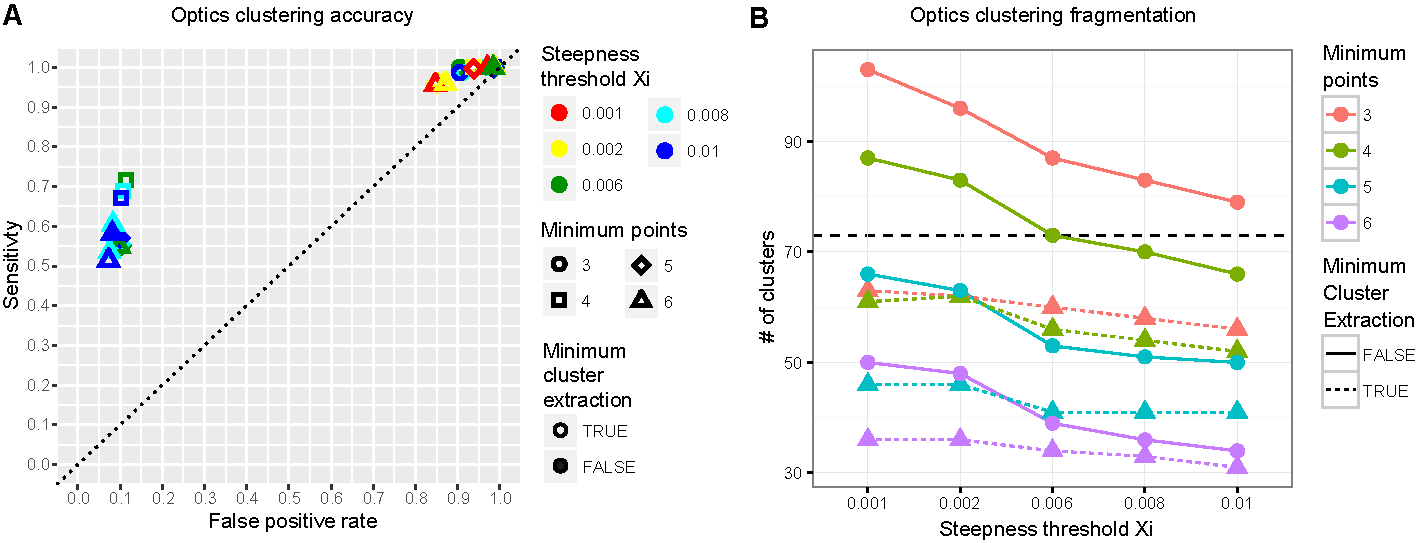
\includegraphics[width=\textwidth]{SF1}
 \caption*{ \textbf{ Figure S1. OPTICS clustering optimisation }\\
Effect of OPTICS parameters on clustering accuracy (\textbf{A}) and amount 
 of clusters (\textbf{B}) from a \dotaligner{} dissimilarity matrix of 580 reference RFAM 
 structures and their dinucleotide-shuffled controls (horizontal dashed line indicates 
 expected amount of clusters, or unique RFAM families). }
\end{figure}


\end{document}
